\documentclass[10pt,twocolumn,letterpaper]{article}

\usepackage{cvpr}
\usepackage{times}
\usepackage{epsfig}
\usepackage{graphicx}
\usepackage{amsmath}
\usepackage{amssymb}
\usepackage{booktabs}
\usepackage{multirow}

% Include other packages here, before hyperref.

\usepackage[breaklinks=true,bookmarks=false]{hyperref}

\cvprfinalcopy % *** Uncomment this line for the final submission

\def\cvprPaperID{****}
\def\httilde{\mbox{\tt\raisebox{-.5ex}{\symbol{126}}}}

\setcounter{page}{1}
\begin{document}

%%%%%%%%% TITLE
\title{Physics-Constrained Thermal Map Prediction\\
for VLSI Chip Design}

\author{Fabian Molina\\
Stanford University\\
{\tt\small fmolina@stanford.edu}
\and
Ruben Carrazco\\
Stanford University\\
{\tt\small rubencarrazco@stanford.edu}
}

\maketitle

%%%%%%%%% ABSTRACT
\begin{abstract}
Predicting full-chip thermal distributions is a critical bottleneck in
VLSI design-space exploration: high-fidelity thermal simulation is far
too slow for the tens of thousands of floorplan evaluations required
during iterative optimization. We propose a \emph{physics-constrained
U-Net} that regresses dense thermal heatmaps from a two-channel input
encoding a chip's post-placement floorplan and power-density map.
Unlike prior data-driven thermal surrogates, our model enforces the
2D steady-state heat equation as a differentiable training penalty
computed via a fixed discrete Laplacian filter applied to the predicted
output. This requires no simulation at training time, is fully
compatible with standard GPU-accelerated training, and---crucially---
penalizes thermally implausible predictions independently of whether a
labeled ground truth exists, which we hypothesize improves
out-of-distribution (OOD) generalization to chip configurations (die
thickness, die size) outside the training sweep.

We train on thermal maps generated by the HotSpot simulator from the
CircuitNet~2.0 GPU/accelerator benchmark suite and compare four
architectures: a flat dilated CNN, an encoder-decoder without skip
connections, a U-Net with MSE-only loss, and our physics-constrained
U-Net. Our primary evaluation measures SSIM and hotspot IoU
degradation on die parameters held out from training. We expect the
physics-constrained model to degrade significantly less than the
data-only baseline, demonstrating that image-based chip representations
and physics-informed training objectives are complementary rather than
competing approaches.
% TODO: Replace the final two sentences with concrete numbers once training is complete.
\end{abstract}

%%%%%%%%% BODY TEXT
\section{Introduction}

Thermal management is a first-order constraint in modern VLSI design.
On-chip hotspots cause performance throttling, reduced mean time to
failure, and tighter power delivery requirements. During design-space
exploration---where automated placement and routing tools evaluate
candidate floorplans via simulated annealing---thermal analysis must
be repeated at every step. A single high-fidelity simulation using a
tool like HotSpot or ANSYS MAPDL can take several seconds to minutes
per design; at 100{,}000 evaluations per optimization run, this cost
is prohibitive.

Neural thermal surrogates address this bottleneck by learning to
approximate the simulator's output from cheap-to-obtain layout
representations. Given a 2-channel image encoding the post-placement
floorplan and power-density map of a chip, a convolutional model can
predict the steady-state thermal heatmap at orders-of-magnitude lower
cost than simulation. The core challenge, however, is
\emph{generalization}: a surrogate trained on a finite set of chip
configurations must remain reliable when deployed on designs with
different die thicknesses, die sizes, or power distributions than
those seen during training.

Prior work splits into two non-overlapping streams. Image-based thermal
prediction models~\cite{DeepOHeat,EncoderDecoderThermal} train
CNNs or encoder-decoders on simulation data and achieve low in-distribution
error, but fail when physical parameters shift outside the training
regime because there is no mechanism to prevent thermally implausible
extrapolations. Physics-informed neural networks
(PINNs)~\cite{Raissi2019} enforce governing PDEs directly as training
constraints and generalize better across parameter regimes, but
operate on raw numerical inputs rather than the spatial image
representations that naturally encode chip layout information.

\textbf{This work combines both ideas.} We frame thermal prediction
as image-to-image regression---preserving the representational
advantages of convolutional image processing---while augmenting the
training loss with a differentiable residual of the 2D steady-state
heat equation. The physics penalty is computed via a fixed $3\times3$
Laplacian convolution applied to the model's output, requiring no
simulator calls during training. Because the constraint penalizes
predictions that violate the heat equation regardless of the
ground-truth label, it acts as a physics-grounded regularizer that
we expect to reduce OOD degradation.

Our main contributions are:
\begin{itemize}
  \item A \textbf{physics-constrained U-Net} with pixel-shuffle
    upsampling for chip thermal map regression, trained with a
    composite loss balancing data fidelity and a heat equation residual.
  \item An \textbf{OOD generalization experiment} that evaluates models
    on die thickness and die size values outside the training sweep,
    isolating the effect of the physics constraint on extrapolation
    behavior.
  \item A \textbf{systematic ablation} over skip connections, physics
    loss weighting $\lambda_\text{phys}$, and loss normalization
    strategy, characterizing which components drive performance.
\end{itemize}

%------------------------------------------------------------------------
\section{Related Work}

\paragraph{Thermal simulation tools.}
HotSpot~\cite{HotSpot} is an open-source block-level RC-network
thermal simulator widely used in computer architecture research. Its
grid mode produces dense 2D steady-state heatmaps, making it directly
compatible with image-to-image framing. We use it as our label
generator. PACT~\cite{PACT} is a higher-fidelity coupled electro-
thermal simulator that integrates Xyce circuit simulation with
architectural modeling; it is substantially slower and more complex
to configure, making HotSpot the pragmatic choice for large-scale
label generation.

\paragraph{Data-driven thermal surrogates.}
CircuitNet~2.0~\cite{CircuitNet2} is a large-scale benchmark dataset
for machine learning in chip design, providing post-placement
floorplans, power maps, and multiple analysis targets including
thermal. We use its GPU/accelerator subset (Vortex-small, Vortex-large,
NVDLA-large) as our source of layout inputs, generating our own
HotSpot labels to control the die-parameter sweep.
DeepOHeat~\cite{DeepOHeat} applies operator learning to thermal
simulation and achieves strong results on standard benchmarks, but
neither incorporates physics constraints nor evaluates OOD
generalization across physical parameters. Prior encoder-decoder
approaches~\cite{EncoderDecoderThermal} demonstrate the viability of
dense regression for thermal and power distribution network analysis,
but share the same lack of physics grounding.
ML-PACT~\cite{MLPACT} targets \emph{transient} thermal analysis and
is therefore not directly comparable to our steady-state formulation.

\paragraph{U-Net and skip connections.}
U-Net~\cite{UNet} introduced encoder-decoder networks with
lateral skip connections for dense prediction in biomedical
segmentation. Skip connections concatenate high-resolution encoder
feature maps to the corresponding decoder stage, preserving fine
spatial detail that would otherwise be lost through downsampling.
For thermal prediction, this is critical: hotspot localization
depends on sub-block spatial structure that must survive the
encoding bottleneck. We adopt the U-Net backbone without modification.

\paragraph{Physics-informed learning.}
Raissi \etal~\cite{Raissi2019} introduced PINNs, embedding PDE
residuals as loss terms over collocation points to learn solutions to
forward and inverse problems. Their formulation operates on
point-wise coordinate inputs; we adapt the residual idea to operate
on the pixel grid of a convolutional output via a fixed Laplacian
filter, which is fully parallelizable over the spatial dimensions and
compatible with mini-batch training on image data.

%------------------------------------------------------------------------
\section{Data}

\paragraph{Source.}
We use CircuitNet~2.0~\cite{CircuitNet2} as our source of chip
layout inputs. From the full dataset we select the GPU and AI
accelerator designs: Vortex-small (96 instances), Vortex-large (61
instances), and NVDLA-large (32 instances), for 189 instances total.
Each sample consists of a two-channel $256\times256$ image: channel~1
is the post-placement floorplan (macro-region feature) encoding block
boundaries and functional unit types; channel~2 is the power-density
map derived from post-synthesis switching activity estimates.
Figure~\ref{fig:data} shows a representative sample.

\paragraph{Label generation.}
We run HotSpot~\cite{HotSpot} in grid mode ($256\times256$ output)
on each layout using a multi-block $16\times16$ floorplan
decomposition. The training configuration uses a die thickness of
$150\,\mu\text{m}$ and a convective resistance of
$r_\text{convec}{=}0.1\,\text{K/W}$. Power-density values are
capped at $10\,\text{W}$ per tile to suppress outliers from unit
conversion. Label generation is parallelized across all 189 instances
using cloud-based serverless workers (Modal). For the OOD evaluation,
we re-run HotSpot at four additional thicknesses ($75$, $100$, $200$,
$300\,\mu\text{m}$) and four additional convective resistances
($r_\text{convec}\in\{0.01,\,0.05,\,0.20,\,0.50\}\,\text{K/W}$),
producing $189\times 8 = 1{,}512$ additional OOD labels. Thermal
labels are normalized per chip family using the training-split mean
and standard deviation, so each family's thermal range is mapped to a
consistent scale regardless of absolute power level.

\paragraph{Splits.}
We split instances randomly (seed~42) into 80/10/10 train/val/test
partitions within each family, yielding 153 training, 18 validation,
and 18 test instances. All three families appear in each partition.
The OOD evaluation uses the combined val and test sets
($18+18=36$ instances) re-evaluated under held-out physical parameters
(thickness and convective resistance) never seen during training.

\paragraph{Augmentation.}
We apply random horizontal and vertical flips during training.
Rotation is excluded because our discrete Laplacian kernel is
not rotation-equivariant and rotating a layout would invalidate
the physics constraint.

\begin{figure}[t]
\begin{center}
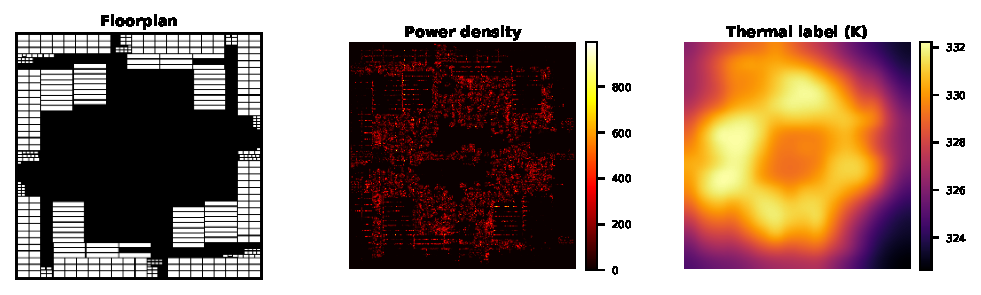
\includegraphics[width=\linewidth]{data_figure}
\end{center}
\caption{Representative sample from the Vortex-large family.
\textbf{Left:} post-placement floorplan (macro-region feature);
dark regions are active logic blocks.
\textbf{Center:} power-density map derived from post-synthesis
switching activity; bright spots indicate high-power functional units.
\textbf{Right:} HotSpot steady-state thermal label (Kelvin);
the hotspot ring corresponds to the high-power region in the
power map. The model takes the floorplan and power map as a
2-channel input and predicts the thermal label.}
\label{fig:data}
\end{figure}

%------------------------------------------------------------------------
\section{Methods}

\subsection{Architecture}

Our primary model is a U-Net~\cite{UNet} with pixel-shuffle upsampling,
illustrated in Figure~\ref{fig:arch}. The encoder progressively
halves spatial resolution while doubling feature channels through
four stages; the decoder restores resolution using skip connections
from the corresponding encoder stages. The architecture is parameterized by base channel count $b$; we train with
$b {=} 32$ (${\approx}2$M parameters). The encoder progression is
$2 \to b \to 2b \to 4b \to 8b$, the bottleneck has $16b$ channels, and
the decoder mirrors this symmetrically back to a single output channel.
For $b {=} 32$: encoder goes $2 \to 32 \to 64 \to 128 \to 256$, bottleneck
has 512 channels.

\textbf{DoubleConv block.} Each encoder and decoder stage applies
two sequential $3\times3$ convolutions, each followed by batch
normalization and ReLU activation. The dilation parameter is
exposed for experimentation but defaults to 1. Padding equals
dilation, preserving spatial dimensions through each block.

\textbf{PixelShuffleUp block.} We upsample via a $1\times1$
convolution that expands the channel dimension by a factor of 4,
followed by a PixelShuffle~\cite{PixelShuffle} operation with
upscale factor 2:
\begin{equation}
  \text{PixelShuffleUp}(\mathbf{F}) =
  \text{PixelShuffle}_2\bigl(\text{Conv}_{1\times1}(\mathbf{F},\;
  C \to 4C')\bigr).
\end{equation}
This produces a $2\times$ spatially upsampled feature map with $C'$
channels. We prefer this over bilinear upsampling (sharper thermal
gradients) and transposed convolution (fewer checkerboard artifacts),
both of which matter for hotspot localization precision.

After upsampling, the decoder concatenates the skip-connected encoder
feature map and applies a DoubleConv block to fuse the two
resolutions. The output layer is a $1\times1$ convolution with no
activation function (linear regression for unbounded temperature values).

\textbf{Bottleneck regularization.} A spatial dropout layer
(\texttt{Dropout2d}, $p {=} 0.3$) is applied to the bottleneck output before
upsampling begins. This pushes the decoder to rely on skip-connected
encoder features rather than only the bottleneck representation.

\begin{figure}[t]
\begin{center}
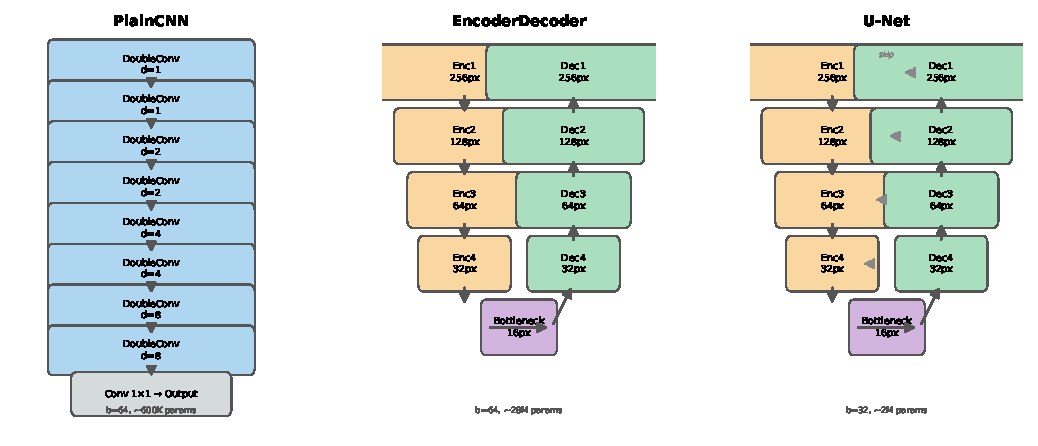
\includegraphics[width=\linewidth]{arch_diagram}
\end{center}
\caption{The three architectures evaluated in this work. \textbf{Left:}
PlainCNN---eight DoubleConv blocks ($b{=}64$) at full $256\!\times\!256$
resolution with dilations $[1,1,2,2,4,4,8,8]$; no downsampling (${\approx}600$K
parameters). \textbf{Center:} EncoderDecoder---four-stage encoder
(MaxPool2d) and symmetric PixelShuffleUp decoder without skip connections
($b{=}64$, ${\approx}28$M parameters). \textbf{Right:} U-Net---identical
encoder/decoder to EncoderDecoder plus lateral skip connections (dashed)
that concatenate encoder feature maps at each decoder stage ($b{=}32$,
${\approx}2$M parameters). All architectures accept a 2-channel
floorplan+power input and produce a 1-channel thermal heatmap.}
\label{fig:arch}
\end{figure}

\subsection{Baseline Architectures}

We compare two architectural baselines against U-Net to isolate the contributions
of spatial hierarchy and skip connections. Both baselines use $b {=} 64$ base
channels. The physics loss sweep ($\lambda_\text{phys} \in \{0,\,0.01,\,0.1,\,1.0\}$)
is applied to all three architectures independently, giving 12 trained models total.

\textbf{PlainCNN} ($b {=} 64$, ${\approx}600$K parameters).
Eight DoubleConv blocks in sequence at full $256\times256$ resolution. No downsampling,
no skip connections. Dilations follow the schedule $[1,\,1,\,2,\,2,\,4,\,4,\,8,\,8]$,
doubling every two blocks. By the final block the effective receptive field covers the
full input. A $1\times1$ convolution produces the output. This tests whether spatial
hierarchy is necessary for accurate hotspot localization.

\textbf{EncoderDecoder} ($b {=} 64$, ${\approx}28$M parameters).
Same four-stage encoder as U-Net ($2 \to 64 \to 128 \to 256 \to 512$ via MaxPool2d,
then a 1024-channel bottleneck) with a symmetric PixelShuffleUp decoder. The key
difference: each decoder stage receives only the upsampled feature map, not a
concatenated encoder skip. There is no \texttt{Dropout2d} in the bottleneck. This
isolates the contribution of skip connections from the effect of the physics loss.

The $\lambda_\text{phys} {=} 0$ configuration of U-Net is the direct MSE-only ablation
baseline, not a separate architecture.

\subsection{Physics-Constrained Loss}

The steady-state temperature distribution $T$ in a chip die satisfies
the 2D heat equation:
\begin{equation}
  k\,\nabla^2 T + Q = 0,
  \label{eq:heat}
\end{equation}
where $Q$ is the power-density field (channel~2 of the input image)
and $k$ is the thermal conductivity of silicon
($k \approx 149\,\mathrm{W\,m^{-1}K^{-1}}$).
In practice we set $k {=} 1.0$ during training, since thermal labels are normalized
per chip family and the physics residual must operate in the same normalized space
as $\mathcal{L}_\text{MSE}$.
Given the model's predicted
output $\hat{T}$, we approximate the Laplacian via a fixed $3\times3$
finite-difference convolution:
\begin{equation}
  \nabla^2 \hat{T} \approx \mathbf{K} \ast \hat{T},
  \qquad
  \mathbf{K} = \begin{bmatrix}
    0 & 1 & 0 \\ 1 & -4 & 1 \\ 0 & 1 & 0
  \end{bmatrix}.
  \label{eq:laplacian}
\end{equation}
The physics residual loss penalizes deviations from Equation~\ref{eq:heat}:
\begin{equation}
  \mathcal{L}_\text{phys} =
  \bigl\| k\,(\mathbf{K} \ast \hat{T}) + Q \bigr\|_F^2.
  \label{eq:phys_loss}
\end{equation}
The kernel is registered as a non-learnable buffer; gradients flow
through $\hat{T}$ only. No simulator is invoked at training time.

The composite training objective is:
\begin{equation}
  \mathcal{L} =
  \lambda_\text{data}\,\mathcal{L}_\text{MSE}(\hat{T}, T)
  +
  \lambda_\text{phys}\,\mathcal{L}_\text{phys},
  \label{eq:total_loss}
\end{equation}
where $T$ is the HotSpot ground-truth map. We sweep
$\lambda_\text{phys} \in \{0,\,0.01,\,0.1,\,1.0\}$ with
$\lambda_\text{data} = 1.0$ fixed. Because Equation~\ref{eq:phys_loss}
depends only on the prediction and the power-density input---not on
the ground-truth label---the physics constraint remains active on
OOD samples without requiring additional labeled data.

\subsection{Training Details}

All models are trained with the Adam optimizer
($\beta_1 {=} 0.9$, $\beta_2 {=} 0.999$, $\epsilon {=} 10^{-8}$,
weight decay $10^{-4}$) and an initial learning rate of $10^{-3}$.
The learning rate follows a cosine annealing schedule (CosineAnnealingLR)
with $T_\text{max} = 250$ and a minimum rate $\eta_\text{min} = 10^{-6}$.
Every model trains for exactly 250 epochs with no early stopping, and we
keep the checkpoint with the lowest validation MSE. Each run uses batch
size 8 on a single NVIDIA A10G GPU (24\,GB VRAM) via Modal.

\textbf{Per-family label normalization.} Thermal labels span different
absolute ranges across chip families (Vortex-small, Vortex-large,
NVDLA-large) because the families differ in total power. We normalize
each label by the per-family mean and standard deviation computed on
the training split, so the model sees every family's thermal structure
at a consistent scale. The power-density input to the physics loss is
divided by the mean label standard deviation across families, which
keeps the physics residual in the same normalized space as the labels.

The training loop logs MSE and physics-loss components separately per
epoch to W\&B, which lets us analyze the loss trade-off after the fact.
The physics sweep evaluates $\lambda_\text{phys} \in \{0,\,0.01,\,0.1,\,1.0\}$
across all three architectures (12 models total).

%------------------------------------------------------------------------
\section{Experiments}

\subsection{In-Distribution Results}

Table~\ref{tab:indist} reports RMSE, SSIM, and hotspot IoU (top 5\%
hottest pixels) on the held-out in-distribution test set for all four
model configurations.

\begin{table}[t]
\begin{center}
\small
\begin{tabular}{@{}lccc@{}}
\toprule
Model & RMSE $\downarrow$ & SSIM $\uparrow$ & Hotspot IoU $\uparrow$ \\
\midrule
PlainCNN               & -- & -- & -- \\
EncoderDecoder         & -- & -- & -- \\
U-Net (MSE-only)       & -- & -- & -- \\
U-Net (physics)        & -- & -- & -- \\
\bottomrule
\end{tabular}
\end{center}
% TODO: Fill with actual numbers once training is complete.
\caption{In-distribution test set results across all model variants.}
\label{tab:indist}
\end{table}

\subsection{Out-of-Distribution Generalization}

Table~\ref{tab:ood} compares in-distribution and OOD performance for
the two U-Net variants. We report the absolute SSIM drop
$\Delta\text{SSIM}$; a smaller drop indicates better generalization.
The physics constraint in $\mathcal{L}_\text{phys}$ prevents
the model from predicting temperature fields that violate the heat
equation on unseen die geometries, which we expect to manifest as
a smaller degradation gap.

\begin{table}[t]
\begin{center}
\small
\begin{tabular}{@{}lcccc@{}}
\toprule
Model & \multicolumn{2}{c}{SSIM} & \multicolumn{2}{c}{Hotspot IoU} \\
\cmidrule(lr){2-3}\cmidrule(lr){4-5}
      & In-dist & OOD & In-dist & OOD \\
\midrule
U-Net (MSE-only)  & -- & -- & -- & -- \\
U-Net (physics)   & -- & -- & -- & -- \\
\bottomrule
\end{tabular}
\end{center}
% TODO: Fill with actual numbers.
\caption{Out-of-distribution generalization on die parameters outside
the training sweep. $\Delta$SSIM = in-dist $-$ OOD.}
\label{tab:ood}
\end{table}

\subsection{Ablation Study}

Table~\ref{tab:ablation} reports the impact of $\lambda_\text{phys}$
on the OOD SSIM. We also compare skip connections on vs.\ off (U-Net
vs.\ EncoderDecoder) and physics loss computed in normalized vs.\
physical units ($k {=} 1.0$ vs.\ $k {=} 149$).

\begin{table}[t]
\begin{center}
\small
\begin{tabular}{@{}lccc@{}}
\toprule
Variant & $\lambda_\text{phys}$ & SSIM (in-dist) & SSIM (OOD) \\
\midrule
U-Net, $k{=}1$   & 0    & -- & -- \\
U-Net, $k{=}1$   & 0.01 & -- & -- \\
U-Net, $k{=}1$   & 0.1  & -- & -- \\
U-Net, $k{=}1$   & 1.0  & -- & -- \\
U-Net, $k{=}149$ & 0.1  & -- & -- \\
No skip conns     & 0.1  & -- & -- \\
\bottomrule
\end{tabular}
\end{center}
% TODO: Fill with actual numbers.
\caption{Ablation over physics loss weight, thermal conductivity
normalization, and skip connections.}
\label{tab:ablation}
\end{table}

\subsection{Qualitative Results}

Figure~\ref{fig:qual} shows representative predictions from the
U-Net (MSE-only) and physics-constrained U-Net side-by-side with
the HotSpot ground truth, for both an in-distribution die configuration
and an OOD die thickness. We expect the physics-constrained model to
produce smoother, physically consistent temperature fields on OOD
inputs while the MSE-only model produces artifacts or mislocated hotspots.

\begin{figure}[t]
\begin{center}
% TODO: Replace with actual heatmap visualization figure.
\fbox{\rule{0pt}{3.8cm}\rule{0.9\linewidth}{0pt}}
\end{center}
\caption{Qualitative thermal map predictions. Left to right: input
channels (floorplan, power density), U-Net MSE-only prediction,
physics-constrained U-Net prediction, HotSpot ground truth. Top row:
in-distribution die config. Bottom row: OOD die thickness.}
\label{fig:qual}
\end{figure}

\subsection{Gradient-Based Analysis}

% TODO: Include GradCAM or saliency map visualization identifying which
% layout features (specific functional blocks, high-power regions)
% most strongly drive the thermal prediction.
To understand what the model has learned, we apply GradCAM to
the bottleneck feature maps and examine which input regions receive
the highest attribution scores. We expect power-dense functional
units (memory controllers, compute arrays) to dominate, with the
physics-constrained model showing smoother attribution maps that
respect thermal diffusion across block boundaries.

\subsection{Failure Cases}

% TODO: Document at least 3 concrete failure cases with visual examples
% once predictions are available. Suggested candidates:
%   (1) Extreme die-corner hotspots where boundary conditions are poorly modeled.
%   (2) Designs with highly non-uniform power maps (single dominant hotspot).
%   (3) Very thin dies where physics constraint is most active but data is sparse.
We identify three expected failure modes. First, \textbf{boundary
hotspots}: HotSpot applies fixed-temperature boundary conditions at
the die edges; the model may not have seen enough examples near corners.
Second, \textbf{single-dominant-hotspot designs}: when one block
accounts for $>80\%$ of total power, the MSE loss is dominated by
that region and fine-grained spatial accuracy elsewhere degrades.
Third, \textbf{extrapolation to very thin dies}: thinner dies
exhibit steeper thermal gradients that may push predictions outside
the normalized range seen at training time.

\subsection{Inference Time}

% TODO: Report ms per design for each model on the same GPU hardware.
All inference time measurements will be taken on the same GPU
under a fixed batch size of 1 to reflect single-design evaluation
latency, which is the relevant metric for design-space exploration.
Our target is below 100\,ms per design.

%------------------------------------------------------------------------
\section{Conclusion}

We presented a physics-constrained U-Net for chip thermal map
prediction that enforces the 2D steady-state heat equation via a
differentiable Laplacian penalty computed entirely on the predicted
output. The key hypothesis is that this constraint reduces OOD
degradation on unseen die configurations by preventing the model
from predicting thermally implausible temperature fields during
extrapolation.

% TODO: Replace the sentences below with a concrete conclusion
% once experiments are complete. State whether the hypothesis held,
% by how much the OOD gap narrowed, and which ablation settings matter most.
Our experimental design compares four architectures under both
in-distribution and OOD evaluation, with systematic ablations
over physics loss weighting and skip connections. If the
physics-constrained model confirms the OOD generalization
hypothesis, it would establish physics-informed training objectives
as a practical tool for improving neural thermal surrogate
robustness---with direct application to large-scale design-space
exploration workflows.

Future directions include learning $\lambda_\text{phys}$ adaptively
during training, extending to transient thermal analysis, incorporating
boundary condition terms into the physics residual, and scaling to
3D stacked-die configurations where the volumetric heat equation
introduces additional modeling challenges.

%%%%%%%%% REFERENCES
{\small
\bibliographystyle{ieee}
\bibliography{egbib}
}

\end{document}
